\documentclass{article}
\usepackage{graphicx} % include figures
\usepackage{xeCJK} % Chinese language support
\usepackage{bm}
\usepackage{amsmath,amsthm,amssymb,amsfonts}
\usepackage{cite}
\usepackage[colorlinks,linkcolor=red,anchorcolor=blue,citecolor=green,CJKbookmarks=true]{hyperref}
\usepackage{indentfirst} % indent before a paragraph, Chinese-style
\usepackage{amsmath}
\usepackage[margin=3.5cm]{geometry}
\usepackage{titlesec}
\usepackage{amsmath}
\usepackage{amssymb}
% \linespread{1.6}
\geometry{left=3.2cm,right=3.2cm,top=3.2cm,bottom=3.2cm}
\usepackage{booktabs}
\usepackage{multirow}
\usepackage{array} % assign height for tables
\usepackage{listings}
\usepackage{xcolor}
\usepackage{ulem}
\usepackage{enumitem}
\usepackage{tikz}
\usepackage{lipsum}
\usepackage{empheq} % enable eq numbering inside a brace
\usepackage{float} % forces figs to appear precisely at the location in code
\usepackage[section]{placeins} % prevents figs appearing after its section

\usepackage{mdframed} % when codes cross pages, this is used to add a frame
\setenumerate[1]{itemsep=0pt,partopsep=0pt,parsep=\parskip,topsep=5pt}
\setitemize[1]{itemsep=0pt,partopsep=0pt,parsep=\parskip,topsep=5pt}
\setdescription{itemsep=0pt,partopsep=0pt,parsep=\parskip,topsep=5pt}
% therom
\makeatletter
\thm@headfont{\sc}
\makeatother
\newtheorem{theorem}{Theorem}

\usepackage{hyperref}% keeps internal links (include table of contents) black
\hypersetup{%
  colorlinks = true,
  linkcolor  = black
}

%%%%%%%%%%%%% MATLAB configuration %%%%%%%%%%%%%
%\usepackage{listings} % used for code highlight
%\lstset{extendedchars=false}%这一条命令可以解决代码跨页时,章节标题,页眉等汉字不显示的问题
%\usepackage[framed,numbered,autolinebreaks]{mcode}
\usepackage[T1]{fontenc}
\usepackage[numbered,framed]{matlab-prettifier}
\usepackage{filecontents}
\let\ph\mlplaceholder % shorter macro
\lstMakeShortInline"
\lstset{
  style              = Matlab-editor,
  basicstyle         = \mlttfamily,
  escapechar         = ",
  mlshowsectionrules = true,
}
\usepackage{physics} % Partial derivative, delta derivative
%\begin{filecontents*}{/code/LIP_straightline.m}

%%%%%%%%%%%% MATLAB configuration %%%%%%%%%%%%%%

%\setCJKmainfont[BoldFont = 黑体]{宋体}
%\setlength{\parindent}{2em} %设置段首空两格
%如果不要缩进 用\noindent

%%%%%%%%%%%%%%%%%%%%%%%%%%%%%%%%%%%%%%%%%%%%%%%%%%%%%%%%%%%%%%%%%%%%%%%%
%%%%%%%%%%%%%%%%%%%%%%%%%%%%%%%%%%%%%%%%%%%%%%%%%%%%%%%%%%%%%%%%%%%%%%%%
%%%%%%%%%%%%%%%%%%%%%%%%%%%%%%%%%%%%%%%%%%%%%%%%%%%%%%%%%%%%%%%%%%%%%%%%
%%%%%%%%%%%%%%%%%%%%          Article             %%%%%%%%%%%%%%%%%%%%%%
%%%%%%%%%%%%%%%%%%%%%%%%%%%%%%%%%%%%%%%%%%%%%%%%%%%%%%%%%%%%%%%%%%%%%%%%
%%%%%%%%%%%%%%%%%%%%%%%%%%%%%%%%%%%%%%%%%%%%%%%%%%%%%%%%%%%%%%%%%%%%%%%%
%%%%%%%%%%%%%%%%%%%%%%%%%%%%%%%%%%%%%%%%%%%%%%%%%%%%%%%%%%%%%%%%%%%%%%%%
\title{ME106 Project12 Report}
\author{\large Rui\hspace{0.5cm}Wang \\ 3033461836}
\date{}
\begin{document}
\maketitle
\vspace{4cm}
\tableofcontents
\clearpage
\section{Problem Restatement}
This problem is an example where Navier-Stokes equation is used. An oscillating plate is moving in the pattern $U = cos(500t)$, where $U$ denotes its velocity. The plate is horizontal and infinitely long, where the domain of fluid is semi-infinite. With additional information, we can solve for the fluid field which varies with time.

Several assumptions have to be made before we can proceed to solve the problem:
\begin{itemize}
  \item The fluid is incompressible
  \item The flow is always laminar
  \item The flow satisfies no-slip boundary conditions
  \item The fluid is Newtonian
  \item Gravity is not taken into consideration
\end{itemize}
There are some other assumptions closely related to the equations themselves. For the sake of convenience and perspicuity, they will be illustrated later in this report.

\section{Part (a). Solve For the Velocity Field}
First we write the Navier-Stokes Equation for this flow field. Then, with proper assumptions, the equation can be solved analytically. Last, we plot the velocity field.

\begin{align}
\pdv{u}{x} + \pdv{v}{y} = 0
  \label{eq:incompressibility}
\end{align}

\begin{align}
\rho ( \pdv{u}{t} + u\pdv{u}{y} + v\pdv{u}{y} ) = -\pdv{P}{x} + \mu (\pdv[2]{u}{x} + \pdv[2]{v}{y})
  \label{eq:N-S1}
\end{align}

\begin{align}
\rho ( \pdv{v}{t} + u\pdv{v}{x} + v\pdv{v}{y} ) = -\pdv{P}{y} + \mu (\pdv[2]{v}{x} + \pdv[2]{v}{y})
  \label{eq:N-S2}
\end{align}

And boundary conditions: no-slip boundary condition
\begin{align}
  u|_{y = 0} = U
  \label{eq:boundary1}
\end{align} where $U = Re[e^{i500t}]$.
Also, the condition that fluid cannot penetrate the wall
\begin{align}
  v|_{y = 0} = 0
  \label{eq:boundary2}
\end{align}

Next we try to simplify these equations by vanishing all zero terms. Since the plate is indefinite, any value cannot vary along the $x$ direction because of symmetry. Therefore, all terms with $x$ will be eliminated. For equation \ref{eq:incompressibility}, we have
\begin{align}
\pdv{u}{x}=0, \pdv{v}{y} = 0
  \label{eq:dvdy=0}
\end{align}

For equation \ref{eq:N-S1} and \ref{eq:N-S2}, also divide every term by $\rho$ thus $\mu$ turns into $\nu$. Therefore we have
\begin{align}
\nu \pdv[2]{u}{y} = \pdv{u}{t} + v \pdv{u}{y}
  \label{eq:NV-1-simplified1}
\end{align}

\begin{align}
\nu \pdv[2]{v}{y} = \pdv{v}{t} + v \pdv{v}{y}
  \label{eq:NV-2-simplified1}
\end{align}

Note that with boundary condition $v|_{y = 0} = 0$, and equation \ref{eq:dvdy=0}, we can integrate and conclude that $v = 0$ throughout the space. Hence the equations can be further simplified into
\begin{align}
\nu \pdv[2]{u}{y} = \pdv{u}{t}
  \label{eq:NV-1-simplified2}
\end{align}

\begin{align}
v = 0 \label{eq:v=0}
\end{align}

These are the equations that we need to solve, and they happen to have a close-form solution. When $t$ is very large and the system has entered a stable(but not steady) state, all fluid particles move in an oscillating manner and the angular frequency is $\omega = 500$. Therefore, we can suppose that the velocity $u$ is of the form

\begin{align}
u = Re[f(y)e^{i500t}] \label{eq:v=0}
\end{align}
where $f(y)$ is some function of $y$. Substitute this expression into equation \ref{eq:NV-1-simplified2}, and we obtain
\begin{align}
\pdv[2]{f}{y} = \frac{500i}{\nu}f \label{eq:fyeq}
\end{align}
The general solution for this 2nd order homogeneous differential equation is 
\begin{align}
f = C_1 e^{\sqrt{500i/\nu}y} + C_2 e^{-\sqrt{500i/\nu}y}\label{eq:generalSoln}
\end{align} where $C_1$ and $C_2$ are two arbitrary constants. Next, we obtain $C_1$ and $C_2$ by applying our boundary condition in \ref{eq:boundary1}. Plugging in $y = 0$, we have
\begin{align}
C_1 + C_2 = 1
\end{align}
 However, by inspection, if $C_1 \neq 0$, then the amplitude of the velocity will go to infinity as $y$ goes to infinity, which cannot be the case for our viscous flow. This is because the viscosity damps the velocity, meaning the momentum cannot diffuse to that far without being damped greatly. Therefore, we get
\begin{align}
C_1 = 0, C_2 = 1
\end{align}
This yields
\begin{align}
f(y) = e^{-\sqrt{500i/\nu}y} \label{eq:fy}
\end{align}

Finally this yields
\begin{align}
u = Re[e^{-\sqrt{500i/\nu}y + i500t}], v = 0
\end{align}

\section{Part (b). Non-dimensionalize the Result}
In this section we want to find two values, $x_0$ and $v_0$ that we can use to non-dimensionalize the final answer. These values should be characteristic velocity and length for this problem.

%For this problem, velocity and length scale are first chosen as the maximum velocity and amplitude of the plate, respectively. However, the amplitude of the plate's oscillating motion is so small that the scale of y looks vary large. Therefore, I also tried a different choice, namely the distance that a fixed point on the plate travels in 1 second.
In my solution, velocity and length scale are chosen as the maximum velocity and amplitude of the plate, respectively. This is because the multiple of these two values are special to the system, and can be perceived intuitively. The scaled velocity shows how fast the fluid is moving compared to the plate. The height shows the distance compared to the motion range of the plate.

Since the plate moves in a harmonic oscillation manner $x = x_0 sin(\omega t+\phi_1)$ with velocity $v = v_0 cos(\omega t+\phi_2)$, we can easily obtain the expression for $x$:
\begin{align}
x = 0.002sin(500t)
\end{align}

%\subsection{Method I}
As such we have $v_0 = 1$ m/s and $x_0 = 0.002 $m. Thus the scaled y-value turns into the multiple of the amplitude and the scaled x-value turns into the multiple of the plate's maximum velocity.

Non-dimensionalize our original equation with the two scales, namely $\hat{u} = \frac{u}{v_0}$ and $\hat{y} = \frac{y}{x_0}$,
and we obtain
\begin{align}
\hat{u} = Re[e^{-\sqrt{i/(500\nu)}\hat{y} + i500t}]
\end{align}
where $\hat{u}$ stands for the non-dimensionalized velocity and $\hat{y}$ stands for the non-dimensionalized height.
%\subsection{Method II}
%For the second method, the distance that a fixed point travels in 1 second is $\frac{8}{\pi} $m, which is around $x'_0 = 2.55$m.
%
%Non-dimensionalize our original equation with the two scales, namely $\hat{u} = \frac{u}{v_0}$ and $\hat{y} = \frac{y}{x'_0}$,
%and we obtain
%\begin{align}
%\hat{u} = Re[e^{-\sqrt{i/\nu}\hat{y} + i500t}]
%\end{align}

\section{Part (c). Plot Velocity versus Height}
In this section, we plot the non-dimensional velocity versus the height in the fluid.

  \begin{figure}[H]
    \centering
    \noindent\makebox[\textwidth][c] 
    {
    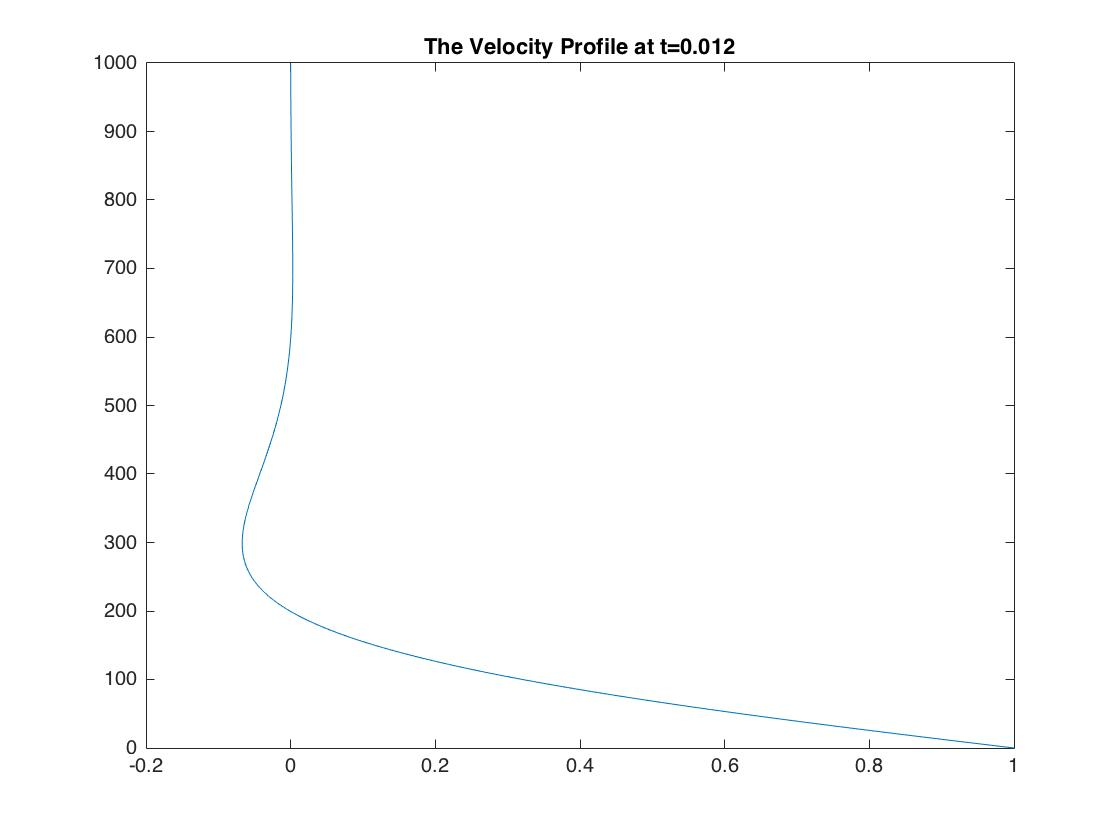
\includegraphics[width=0.5\paperwidth]{images/00.jpg}
    }
    \caption{The Scaled Velocity Profile at t=0.} \label{fig:00}
  \end{figure}
  
  \begin{figure}[H]
    \centering
    \noindent\makebox[\textwidth][c] 
    {
    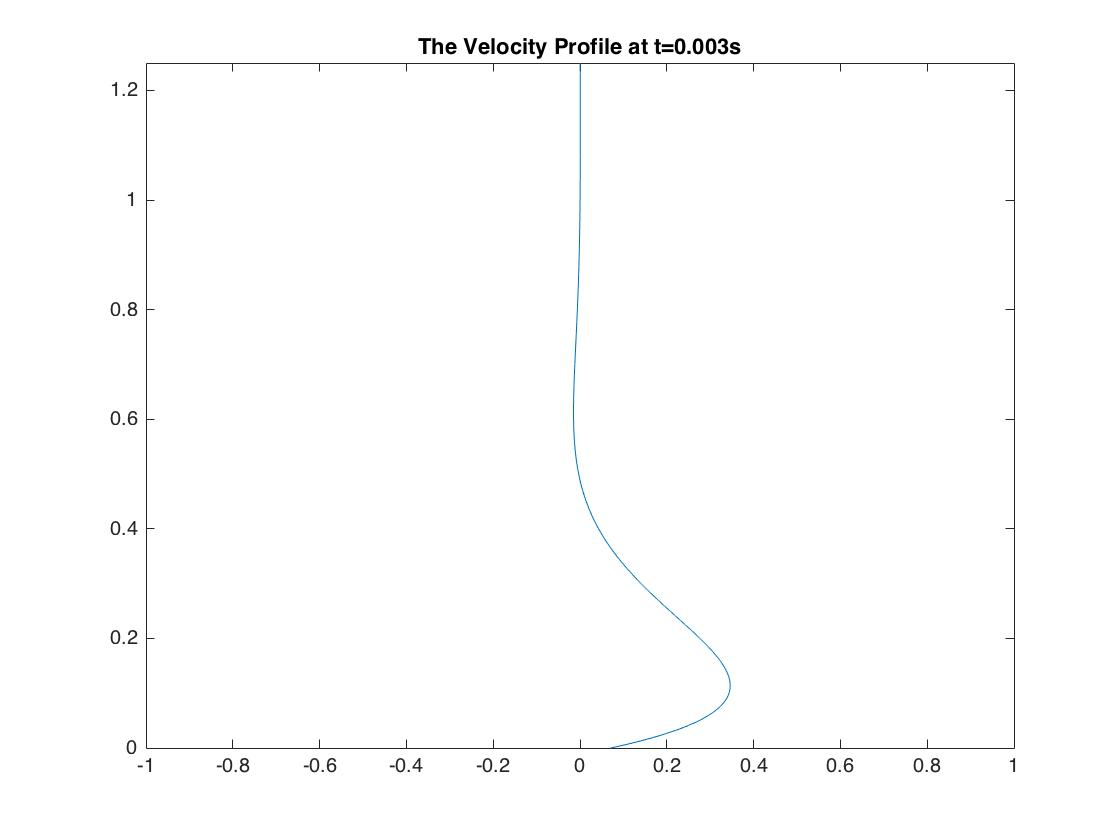
\includegraphics[width=0.5\paperwidth]{images/11.jpg}
    }
    \caption{The Scaled Velocity Profile at t=0.003.} \label{fig:11}
  \end{figure}
  
  \begin{figure}[H]
    \centering
    \noindent\makebox[\textwidth][c] 
    {
    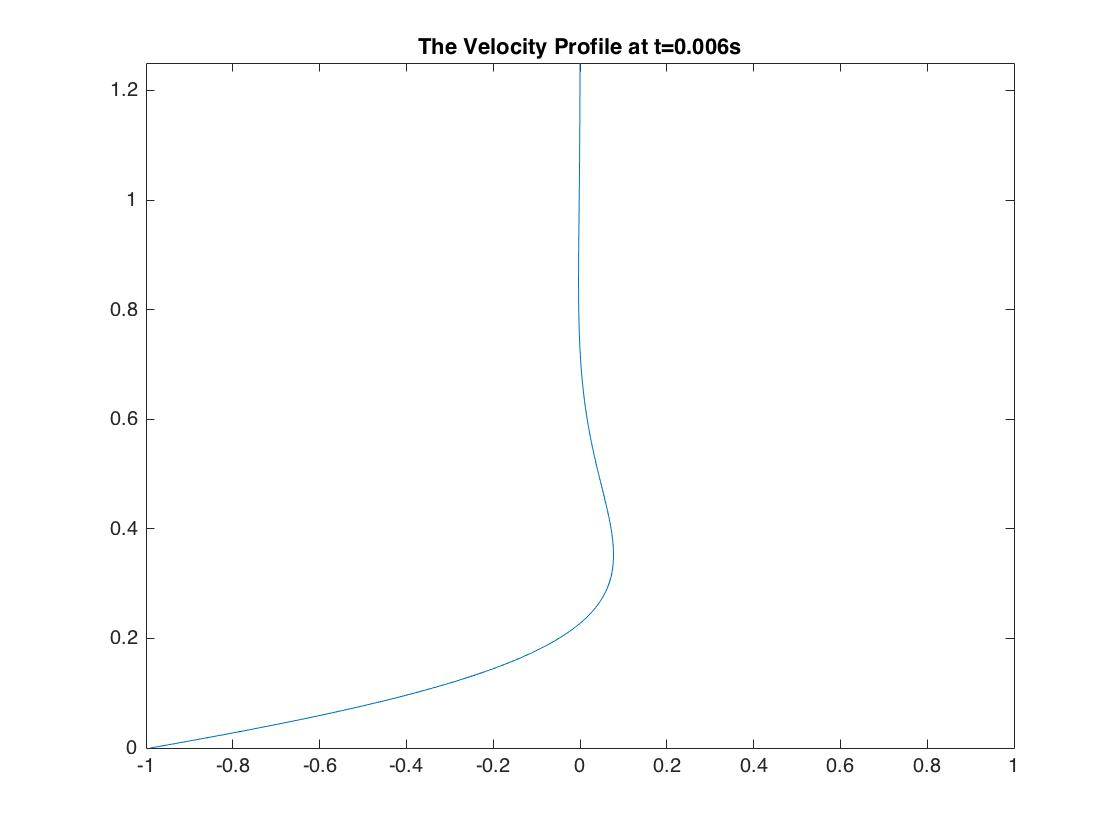
\includegraphics[width=0.5\paperwidth]{images/22.jpg}
    }
    \caption{The Scaled Velocity Profile at t=0.006.} \label{fig:22}
  \end{figure}
  
  \begin{figure}[H]
    \centering
    \noindent\makebox[\textwidth][c] 
    {
    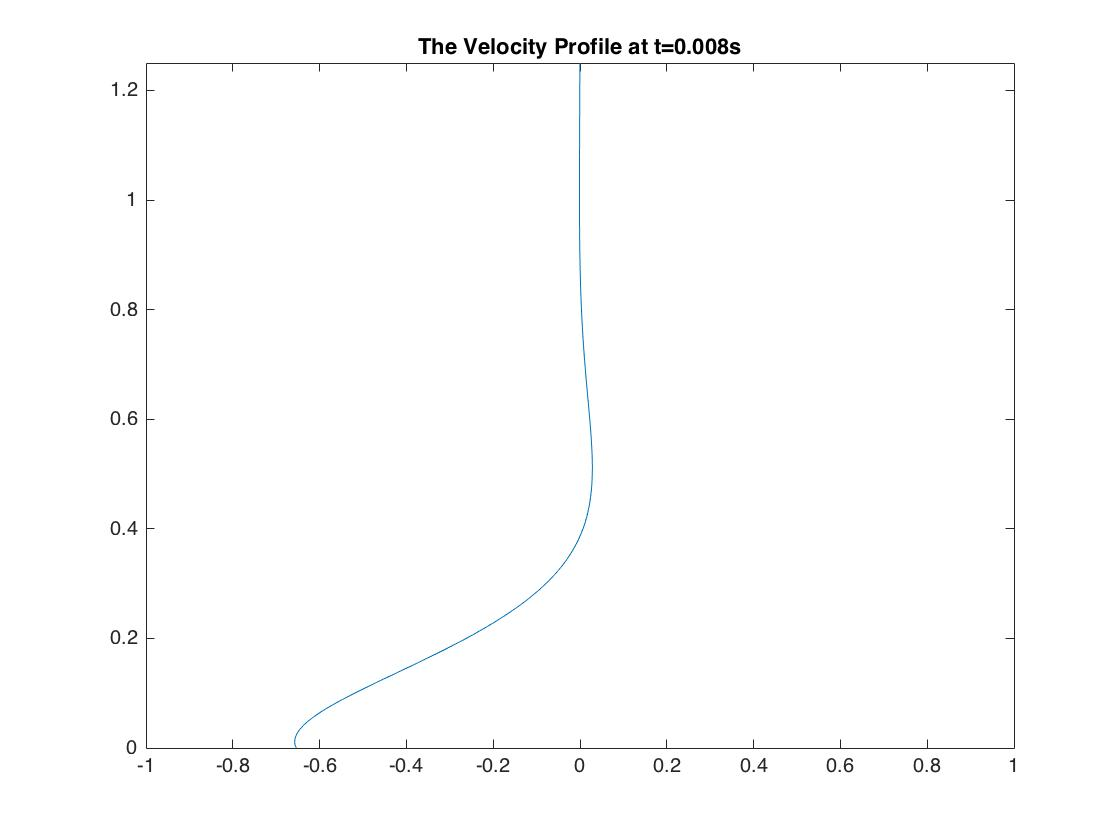
\includegraphics[width=0.5\paperwidth]{images/33.jpg}
    }
    \caption{The Scaled Velocity Profile at t=0.008.} \label{fig:33}
  \end{figure}
  
  \begin{figure}[H]
    \centering
    \noindent\makebox[\textwidth][c] 
    {
    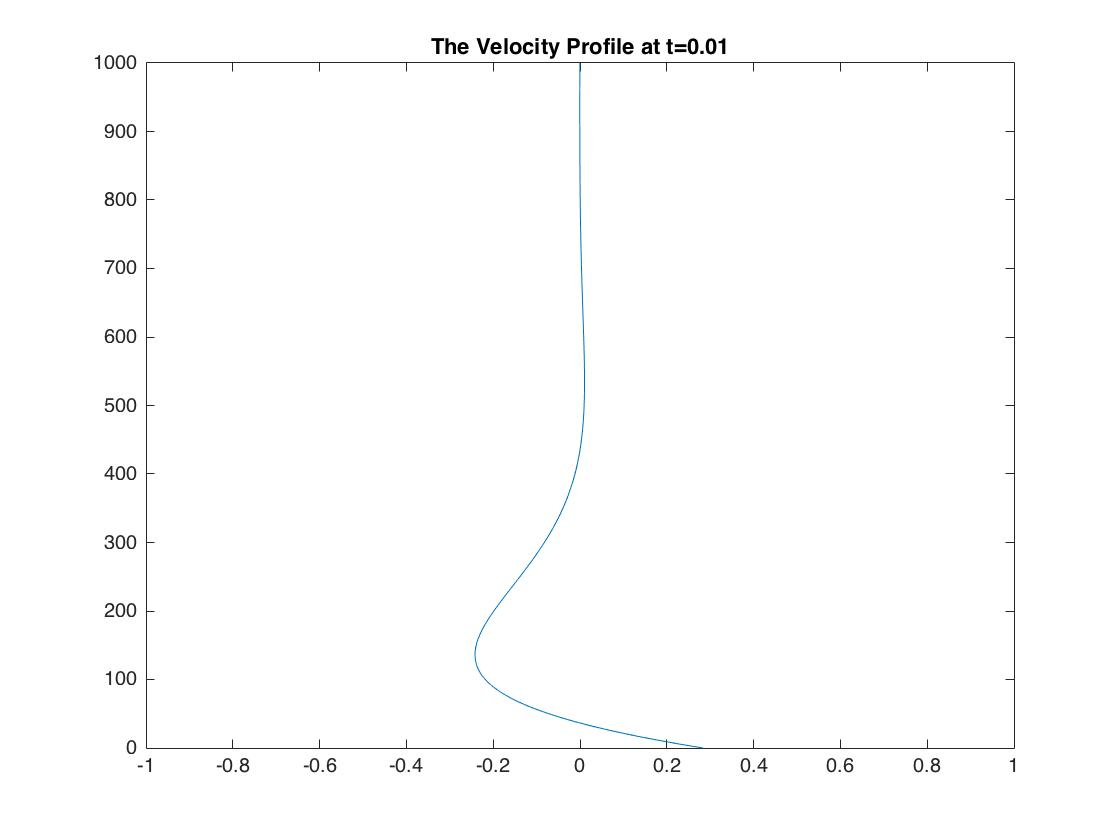
\includegraphics[width=0.5\paperwidth]{images/44.jpg}
    }
    \caption{The Scaled Velocity Profile at t=0.01.} \label{fig:44}
  \end{figure}
  
  Combining them together into one graph, we can get an idea of how the velocity evolves with time.
  \begin{figure}[H]
    \centering
    \noindent\makebox[\textwidth][c] 
    {
    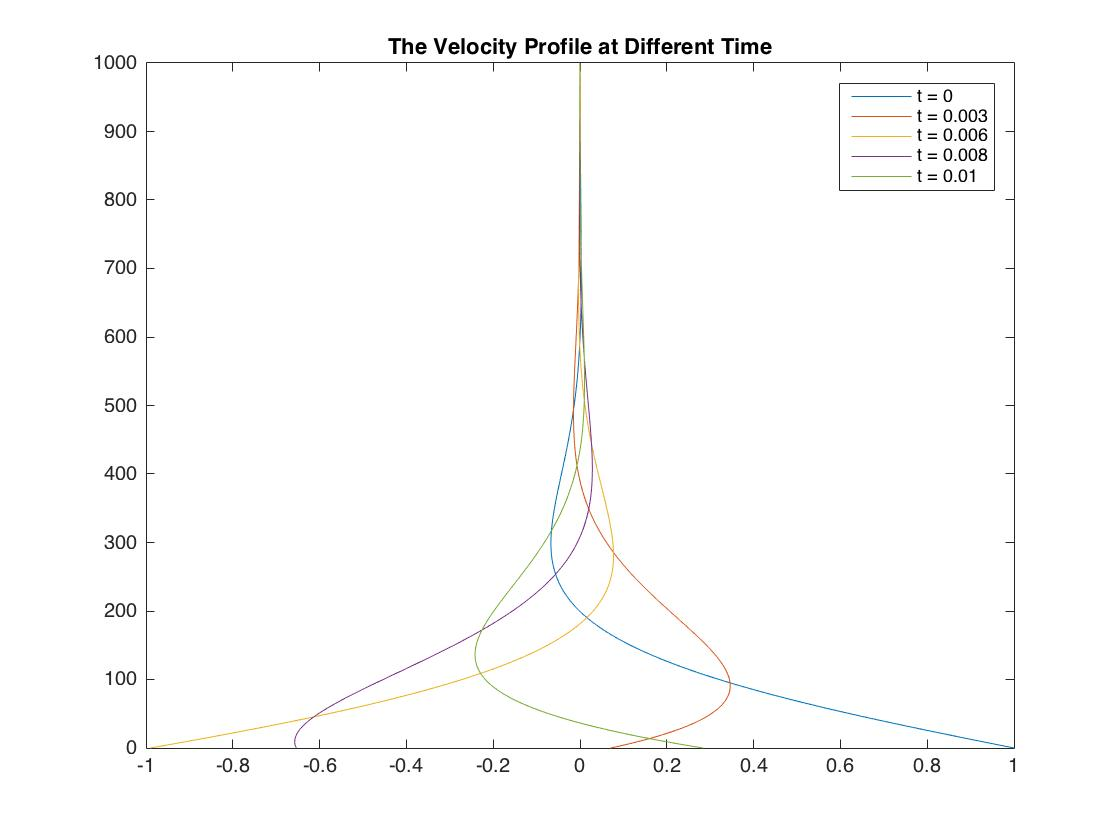
\includegraphics[width=0.5\paperwidth]{images/plotAll.jpg}
    }
    \caption{All plots combined} \label{fig:all}
  \end{figure}
  
  From these plots we can see some features that reflect the physical significances of it. The magnitude of the velocity is the same as the velocity of plate due to no-slip boundary condition, and is often relatively high when $y$ is \textbf{relatively} small. $y$ takes the scale of hundreds because the plate is oscillating very fast and the amplitude is small. In this case the oscillation can spread to far away, till $y = 700$ before it fades away. However, in this specific setting, the velocity of the plate goes to zero well before 2m away, meaning that the viscosity of the fluid has a significant damping effect placed on it. Fluid very far away will not be affected by the oscillation of the plate and will remain still. Also, the velocity profile evolves in a periodic pattern, which is obvious from our equation. This is also due to the fact that the plate is moving periodically, and the viscosity of the fluid ensures that previous motion of fluid particles, compared to the motion of the plate, exerts smaller influence on the current motion of fluid particles.

\clearpage
\appendix
Appendix:
The code for plotting is as follows.
Below is the code to plot everything at different time on the same graph.
\lstinputlisting[style=Matlab-editor]{code/NS.m}

%NOT SURE whether the scale is chosen correctly! ASK RACHEL!
%add code and explanation for the code.

%  \subsection{Problem Statement}
%  \lstinputlisting[style=Matlab-editor, caption = {Commands to plot a velocity field.}]{code/quiverPlot.m}
%  Figure \ref{fig:vel} is the plot for the velocity field.
%  \begin{figure}[H]
%    \centering
%    \noindent\makebox[\textwidth][c] 
%    {
%    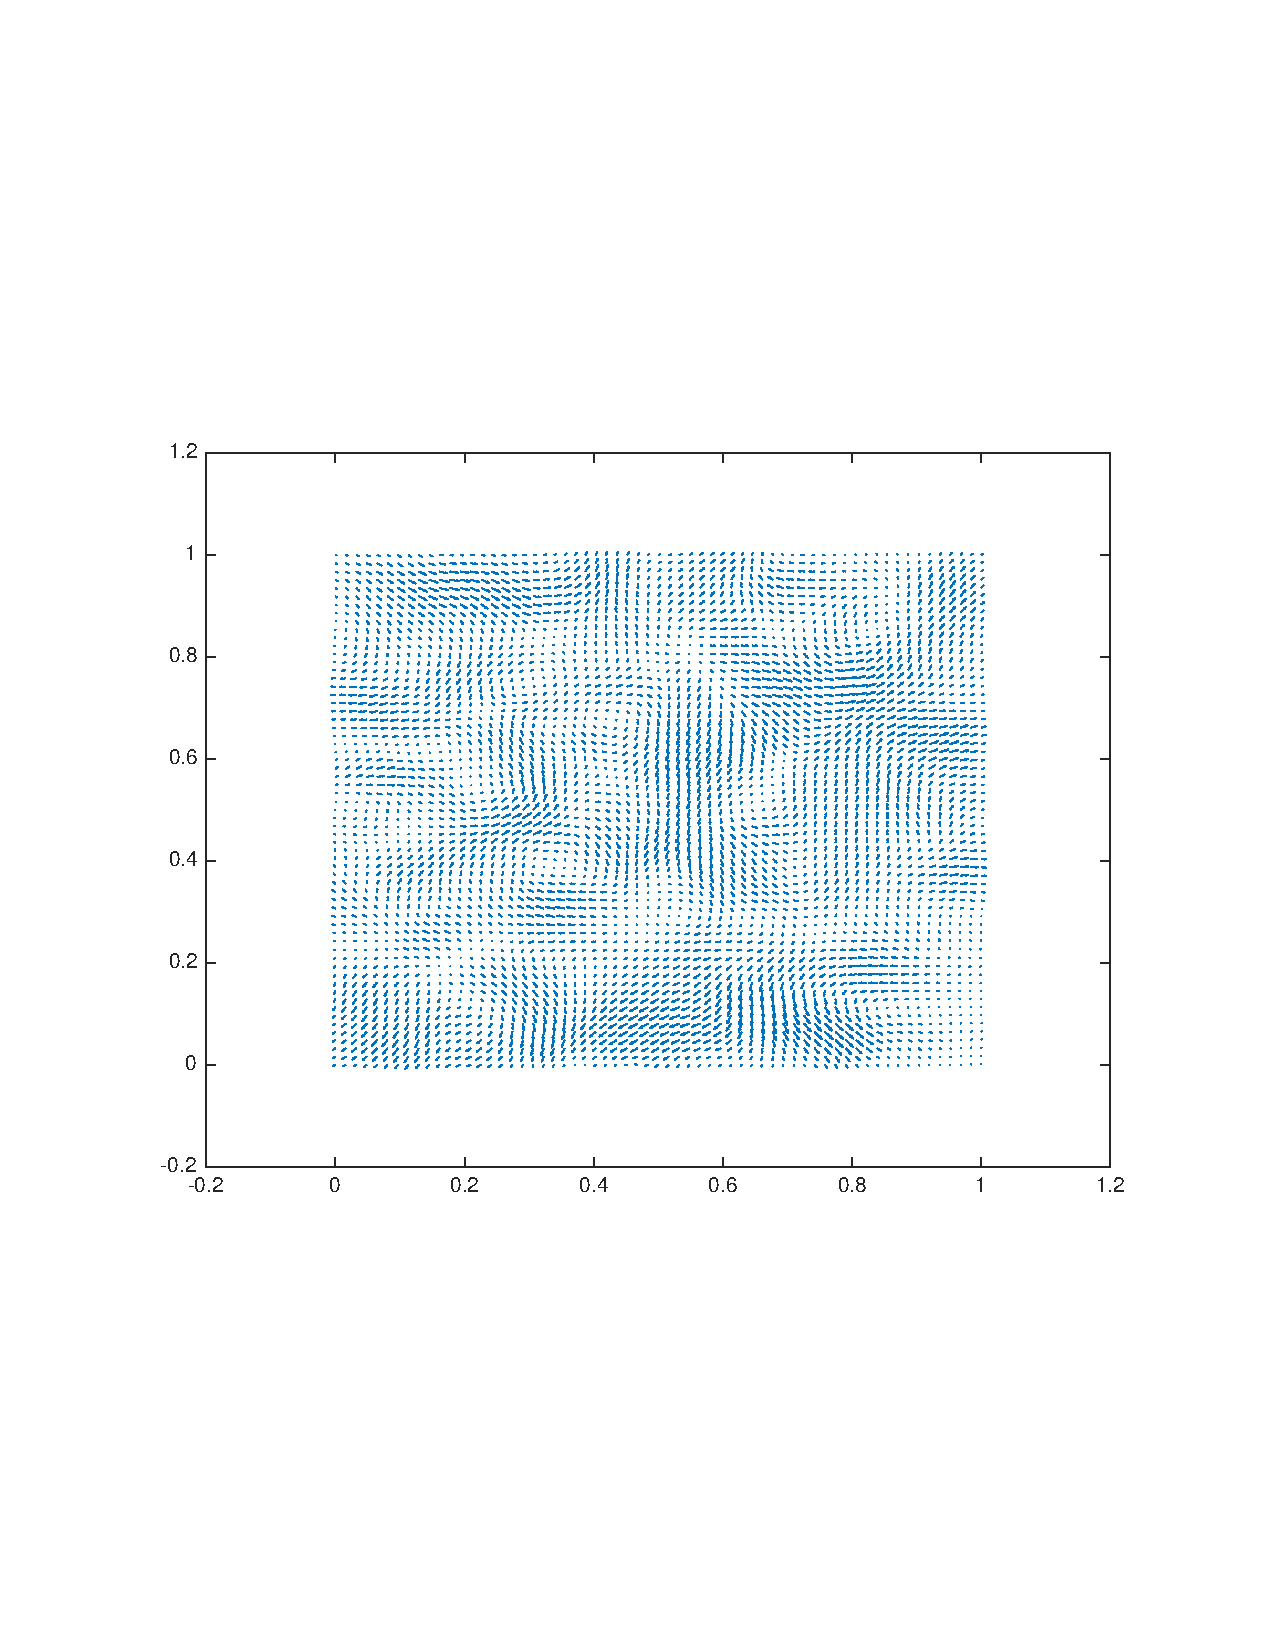
\includegraphics[width=0.5\paperwidth]{images/velocity.pdf}
%    }
%    \caption{The original velocity field.} \label{fig:vel}
%  \end{figure}
  
% print all figures above before new a page
%\appendix
%Appendix:
%
%\lstinputlisting[style=Matlab-editor, caption = {RLCdynamics.m}]{code/RLCdynamics.m}
    %%%%%%%%%%%%%%%
    %%%%%%%%%%%%%%%
    %  CODE HERE  %
    %%%%%%%%%%%%%%%
    %%%%%%%%%%%%%%%
%\lstinputlisting[style=Matlab-editor]{code/RLCdynamics.m}

\end{document}